\documentclass[tikz,margin=2mm]{standalone}

\newcommand*{\m}{\mathsf{m}}

\usetikzlibrary{trees,arrows}

% Define a command for drawing a square
\newcommand{\drawSquare}[2]{
    \fill[black] (#1) rectangle ++(#2,#2); % position, size
}
\begin{document}
  		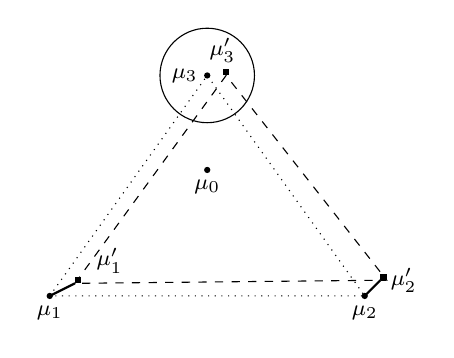
\begin{tikzpicture}[domain=0.001:1, scale=4, xscale=1,font=\footnotesize] 
         


  		%% vertices
    	\draw[-, thick, ] (0,0) node[below]{$\mu_1$} -- (0.08,0.04) node[above, xshift=0.44cm] {$\mu_1'$}; 
		\drawSquare{0.08,0.04}{0.02};	

    	\draw[-, thick, ] (1,0) node[below]{$\mu_2$} -- (1.05,0.05) node[right] {$\mu_2'$};
		\drawSquare{1.05,0.05}{0.02};	

    	
        \fill[black] (0.5,0.4) node[below]{$\mu_0$} circle (0.01);
        \fill[black] (0.5,0.7) node[left]{$\mu_3$} circle (0.01);
        
    	\draw[] (0.62,0.78) node[left]{$\mu_3'$};
        
 		\drawSquare{0.55,0.70}{0.02};	
        
		\fill[black] (0,0) circle (0.01);
		\fill[black] (1,0) circle (0.01);
    	\draw[] (0.5,0.7) circle (0.15);
    	
        \draw[, dotted] (0,0) -- (0.5,0.7) -- (1,0) -- (0,0) ;
        \draw[dashed] (0.08,0.04) -- (0.56,0.70) -- (1.07,0.05) -- (0.08,0.04)  ;


    	\end{tikzpicture}
       	
\end{document}